\section{Metody numeryczne}
\subsection{Metoda macierzy przejścia}
Metoda macierzy przejścia, w skróce nazywana TMM (ang. transfer matrix method) jest używana w optyce i akustyce do analizy propagacji fal odpowiednio elektromagnetycznych i dzwiękowych przez ośrodki warstwowe. Metoda macierzy przejścia może być wykorzystywana do modelowania współczynników transmisji i odbicia w układach liniowych niezmienniczych ze wzlgędu na przesunięcia w kierunku prostopadłym do granicy ośrodków.

W elektromagnetyzmie, macierz przejścia dowolnego układu optycznego wiąże ze sobą amplitudy pól padających i wychodzących \cite{teich1991fundamentals,markos2008wave}:
\begin{equation}
\begin{bmatrix}
U_i \\ 
U_r
\end{bmatrix}
= M 
\begin{bmatrix}
U_t \\
U_b
\end{bmatrix},
\label{eq:tmm}
\end{equation}
gdzie $M$ jest macierzą przejścia układu, $U$ jedt dowolną wybraną skłądową pola elektrycznego lub magnetycznego, odpowiednio $U_i$ - padającą, $U_r$ - odbitą, $U_t$ - transmitowaną przez układ, oraz $U_b$ padającą  z przeciwnej strony. Graficznie sytuację opisywaną powyższym równaniem przedstawia schemat na rysunku \ref{fig:tmm-simple}.

\begin{SCfigure}
	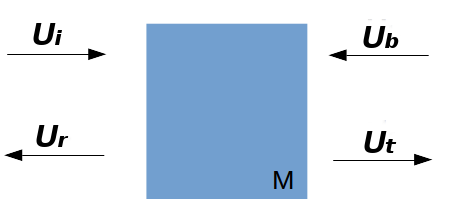
\includegraphics[width=0.6\textwidth]{images/tmm.png}
	\caption{Ilustracja podstawowego elemntu w symulacjach metodą TMM, wraz z ilustracją amplitud z równanie (\ref{eq:tmm}) }
	\label{fig:tmm-simple}
\end{SCfigure}

W przypadku analizy układu złożonego z wielu warstw, oznaczenia z wzoru (\ref{eq:tmm}), możemy poprzez indeks liczbowy przypisać osobno do każdej z macierzy $M_i$:
\begin{equation}
\begin{bmatrix}
U_i^1 \\ 
U_r^1
\end{bmatrix}
= M_1 
\begin{bmatrix}
U_t^1 \\
U_b^1
\end{bmatrix},
\label{eq:tmm-1l}
\end{equation}

\begin{equation}
	\begin{bmatrix}
	U_i^2 \\ 
	U_r^2
	\end{bmatrix}
	= M_2 
	\begin{bmatrix}
	U_t^2 \\
	U_b^2
	\end{bmatrix},
\label{eq:tmm-2l}
\end{equation}

dodając kolejne warstwy np. po lewej stronie od warstwy z rysunku \ref{fig:tmm-simple}, wtedy obliczone $U_i^1$ i $U_r^1$ według wzoru \ref{eq:tmm-1l} dla kolejnej warstwy mają znacznie odpowiednio $U_t^2$ i $U_b^2$. Podstawiając to do wzoru \ref{eq:tmm-2l} otrzymujemy 
\begin{equation}
\begin{bmatrix}
U_i^2 \\ 
U_r^2
\end{bmatrix}
=M_2 M_1 
\begin{bmatrix}
U_t^1 \\
U_b^1
\end{bmatrix},
\label{eq:tmm-2ls}
\end{equation}

Z czego wynika, że w układ złożony z i warstw opisywanych macierzami przejscia $M_i$ można traktować jak jeden element opisywany za pomocą macierzy przejścia będącej iloczynem macierzy opisujących wszystkie jego elementy $M= M_i \cdot M_{i-1} ... \cdot M_1$. Podstawowymi macierzami przejścia wykorzystywanymi do obliczeń w układach warstwowych są
\begin{itemize}
\item Macierz przejścia odpowiadająca propagacji w ośrodku jednorodnym 
\begin{equation}
	M_p=
	\begin{bmatrix}
	\textrm{exp}(-2i\pi k z_0) & 0 \\
	0	&\textrm{exp}(-2i\pi k z_0)\\
	\end{bmatrix},gdzie
\end{equation}
$k$ jest długością wektora falowego w ośrodku w którym zachodzi propagacja w kierunku równoległym do grubości warstwy, a $z_0$ jest grubością warstwy.
\item Macierz opisująca przejście fali E-M przez granicę ośrodków
\begin{equation}
	M_i=\frac{1}{1+r}
	\begin{bmatrix}
	1 & r \\
	r & 1\\
	\end{bmatrix},
\end{equation}
gdzie $r$ jest amplitudowym współczynnikiem odbicia fali na opisywanej granicy ośrodków wynikającym z równań Fresnela i zależnym od kąta padania. 
\end{itemize}

Obliczenie współczynnika transmisji płytki płasko-równoległej wymaga więc skonstruowania macierzy opisującej taką płytkę z trzech macierzy: 
\[
M=M_i \cdot M_p \cdot  M_i.
\]

\subsection{FDTD}
\label{subart:fdtd}
Metoda różnic skończonych w~dziedzinie czasu (ang. FDTD - finite-difference time-domain) jest szeroko wykorzystywana w~niniejszej pracy ze względu na możliwości symulowania ośrodków materialnych opisywanych modelem Lorenza-Drudego \ref{subart:lorenz-drude}, oraz bezpośrednie obliczanie wartości pól $E$ i~$H$ we wszystkich punktach siatki obliczeniowej. Poniżej przedstawione zostały podstawowe elementy tej metody symulacji numerycznych.
Podstawą do współcześnie prowadzonych symulacji elektromagnetycznych w~dziedzinie czasu jest algorytm Yee\cite{1966ITAP14302Y}, który rozwiązywanie równań Maxwella sprowadza do następującej sekwencji:
\begin{enumerate}
\item Zastąpienie wszystkich pochodnych cząstkowych w~prawach Ampera i~Faradaya różnicami skończonymi.
\item Przekształcenie powstałych równań, tak aby wyrazić amplitudy pól $E$ i~$H$ w~nieznanym czasie $t_0 +  \Delta_t$ przez ich wartości w~czasie $t_0$, oraz wartości drugiego pola w~czasie $t_0+ \frac{\Delta_t}{2}$.
\item Obliczyć wartości pola $H$ w~czasie $t_0 +  \Delta_t$.
\item Na podstawie już obliczonych wartości $H$ dla $t=t_0+  \Delta_t$, obliczyć wartości pola $E$ w~czasie $t_0 + \frac{3}{2} \Delta_t$.
\item Powtarzając kroki 3-4 ewoluować stan układu przez żądany czas.
\end{enumerate}A
Przeanalizowany poniżej przykład pozwoli nam lepiej zrozumieć te kilka abstrakcyjnie opisanych kroków. Ponieważ prowadzenie rachunków dla problemu trójwymiarowego byłoby przesadnie skomplikowane, dla celów poglądowych skupimy się na problemie jednowymiarowym.

\subsection{FDTD w~jednym wymiarze}

Załóżmy, że pole elektryczne posiada jedynie składową w~kieruku $z$, w~jedowymiarowej przestrzeni opisywanej przez oś x ($\vec{E}=E_z \cdot \hat{e_z}$). W takiej sytuacji prawo Faradaya możemy zapisać jako:
\begin{equation}
\mu \frac{\partial \vec{H}}{\partial t}= \mu \frac{\partial H_y}{\partial t} \hat{e_y}= \nabla \times \vec{E} = - \frac{\partial E_z}{\partial x} \hat{e_y} 
\label{eq:fdtd-faraday}
\end{equation}
Zgodnie z~oczekiwaniami jedyną zmianną w~czasie składową natężenia pola magnetycznego jest $H_y$. Wykorzystując ten fakt możemy również uprościć zapis prawa Ampera:
\begin{equation}
\varepsilon \frac{\partial \vec{E}}{\partial t}=\nabla \times \vec{H} = \frac{\partial H_y}{\partial x} \hat{e_z}
\label{eq:fdtd-amper}
\end{equation}
Z powyższych równań możemy zapisać  skalarny układ równań różniczkowych na składowe $H_y$ i~$E_z$,
\begin{equation}
\mu \frac{\partial H_y}{\partial t}=\frac{\partial E_z}{\partial x} ,
\varepsilon \frac{\partial E_z}{\partial t}=\frac{\partial H_y}{\partial x},
\end{equation} w~którym zmiana w~czasie amplitudy jednego z~pól wyrażona jest przez pochodną względem $x$ drugiego pola. Równanie wyprowadzone z~\ref{eq:fdtd-faraday} posłuży nam do wyznaczenia zmiany w~czasie natężenia pola magnetycznego, natomiast równanie \ref{eq:fdtd-amper} do obliczenia przyszłych (w czasie $t_0 + \Delta_t$) wartości pola $E$.

\begin{figure}[tb]
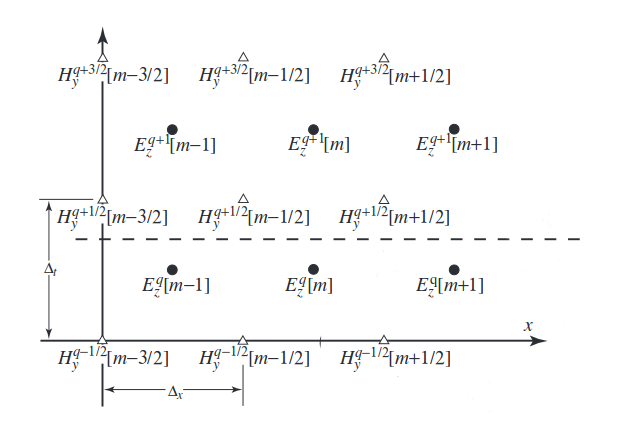
\includegraphics[width=.9\textwidth]{subart/fdtd/leapfrog.png}
\caption{Graficzna prezentacja dyskretyzacji w~jednowymiarowej metodzie FDTD. Pozioma przerywana linia wskazuje przykładową granicę pomiędzy wartościami już obliczonymi i~szukanymi w~kolejnym kroku symulacji. }
\label{pic:leapfrog}
\end{figure}


Dla analizy numerycznych aspektów metody FDTD wygodnie jest traktować czas jako drugi wymiar problemu. Wprowadzając konwencję przypiswania górnych indeksów $q$  iteracjom algorytmu , oraz umieszczanych w~nawiasach kwadratowych indeksów m opisujących położenie w~przestrzeni, możemy wyprowadzić formuły do obliczania wartości obu pól
\begin{equation}
H_y^{q+\frac{1}{2}}[m+\frac{1}{2}]=H_y^{q-\frac{1}{2}}+\frac{\Delta_t}{\mu \Delta_x}(E^q_z[m+1]-E^q_z[m]),
\label{eq:numhy-1dfdtd}
\end{equation}

\begin{equation}
E_z^{q+1}[m]=E_z^{q}+\frac{\Delta_t}{\varepsilon \Delta_x}(H^{q+\frac{1}{2}}_z[m+\frac{1}{2}]-H^{q-\frac{1}{2}}_z[m-\frac{1}{2}]),
\label{eq:numez-1dfdtd}
\end{equation}
 Ponieważ wartości obu pól w~kolejnym korku czasowym wyrażane są jedynie przez wartość tego pola w~kroku poprzednim, oraz wartości drugiego pola w~somsiednich punktach, możemy zastosować dyskretyzację skokową\footnote{Często spotykana jest również nazwa żabi skok, będąca kalką językową z~angielskiego leap-frog}. Jej zastosowanie powoduje, że obliczane wartości pól $E$ i~$H$ nie dotyczą dokładnie tej samej chwili w~czasie, przez co dokładne uzgodnienie fazy obu pól wymaga wykonania dodatkowego ,,połówkowego'' kroku na jednym z~pól. Zaletą takiej dyskretyzacji jest natomiast wyższa - drugiego rzędu, dokładność numeryczna. Ze względu na zysk numeryczny, algorytm skokowy stosujemy również dla dyskretyzacji względem położenia. Graficzną reprezentację rozwiązywania jednowymiarowego problemu elektromagnetycznego metodą FDTD przedstawia rysunek \ref{pic:leapfrog}.

Współczynniki $\frac{\Delta_t}{\varepsilon \Delta_x}$ i~$\frac{\Delta_t}{\mu \Delta_x}$ odgrywają kluczową rolę w~równaniach \ref{eq:numhy-1dfdtd} i~\ref{eq:numez-1dfdtd}, wygodnie jest przedstawić je w~formie pozwalającej przeanalizować jak daleko energia może propagować się w~pojedynczym kroku czasowym \cite{understanding-fdtd}. W tym celu wprowadza się tzw. współczynnik Couranta, $S=\frac{c \Delta_t}{\Delta_x}$, będący stosunkiem odległości pokonywanej przez front fali elektromagnetycznej w~jednym kroku czasowym i~gęstości próbkowania w~przestrzeni. W przypadku symulacji jednowymiarowych, uwzględniając fakt, że wartości w~kolejnych chwilach czasu zależą jedynie od punktów dyskretnych z~najbliższego otoczenia możemy stwierdzić, że współczynnik Couranta powinien spełniać warunek $S\le1$. W szczególności optymalnym dla omawianej sytuacji jest wybranie $S=1$, ponieważ wtedy w~jednym kroku czasowym front fali elektromagnetycznej pokonuje odległość równą $\Delta_x$. Wybranie właściwego współczynnika Couranta komplikuje wprowadzenie niejednorodności w~obszarze symulacji. Ponieważ prędkość fazowa zależy od współczynnika załamania, przy zachowaniu równomiernego próbkowania przestrzennego doprowadzenie do idealnego dopasowania siatki przestrzennej i~kroku czasowego może okazać się niemożliwe, co prowadzi do powstania ,,dyspersji numerycznej'' na siatce FDTD. 

W ogólności dla problemów wielowymiarowych stosuje się wzór
\begin{equation}
S\le\frac{n_{min}}{\sqrt{DIM}},
\label{eq:courant}
\end{equation}
gdzie przez $DIM$ oznaczono liczbę wymiarów przestrzennych symulacji, a $n_{min}$ najniższy współczynnik załamania materiału znajdującego się w~przestrzeni symulacji. Wyznaczenie odpowiedniego współczynnik Couranta dla symulacji z~materiałami dyspersyjnymi (szerzej omówionymi w~części \ref{subart:lorenz-drude}) jest zagadanieniem skomplikowanym, wymagającym każdorazowego rozpatrzenia parametrów symylacji.

\subsection{Warunki brzegowe}
Równania \ref{eq:numhy-1dfdtd} i~\ref{eq:numez-1dfdtd} mogą być oczywiście zastosowane jedynie do punktów nie będących granicą obszaru symulacji. Numeryczne rozwiązanie równania różniczkowego zawsze wiąże się z~odpowiednim dobraniem warunków brzegowych, które nie powinny wprowadzać dodatkowych artefaktów do modelowanego zjawiska. Najprosztszym sposobem jest zastosowanie warunku Dirichleta przyjęcie brzegowych wartości pola elektrycznego lub magnetycznego jako równych 0. Fizycznie wprowadzenie tego typu założenia jest równoważne z~umieszczeniem na granicy symulowanego obszaru idealnego przewodnika, odpowiednio elektrycznego~(PEC)\footnote{Od ang. Perfect Electric Conductor} lub magnetycznego~(PMC)\footnote{Dla wygody numerycznej wprowadza się również przewodniość magnetyczną( W skrócie określanym jako PMC od ang. Perfect Magnetic Conductor)}. Wprowadzenie stałej, równej zero wartości na granicy obszaru symulacji powoduje odbicie obu pól, w~stosunku do pola dla którego ustalono zerową wartość na granicy przy odbiciu następuje zmiana znaku. Przykład wyników symulacji w~pustej przestrzeni ze sztywnymi warunkami brzegowymi znajduje się na ilustracji~\ref{fig:wstep-pml-bad}. Ograniczenie obszaru symulacji za pomocą idealnego przewodnika, de facto ogranicza możliwości metody do modelowania jedynie wnęk rezonansowych. Natomiast większość zjawisk elektromagnetycznych odbywa się w~otwartej przestrzeni \footnote{Za którą z~dobrym przybliżeniem możemy uważać nawet zamknięte laboratorium. Ponieważ analizowane zjawiska dyfrakcji, czy rozpraszania zachodzą w~małym obszarze, położonym z~dala od ograniczeń fizycznych takich jak ściany które słabo odbijają światło widzialne.}.

W przypadku niektórych struktur istnieje naturalne zakończenie obszaru symulacji. Przykładem mogą być periodyczne kryształy fotoniczne, dla których obszar symulacji stanowi komórka elementarna z~periodycznie zadanymi warunkami brzegowymi. Rozwiązania niektórych problemów elektromagnetycznych szybko zanikają w~przestrzeni, w~związku z~czym zastosowanie odpowiednio dużego obszaru symulacji może umożliwić przeprowadzenie obliczeń. Inne zagadnienia wymagają zamiany zmiennych  jak np. $\hat{x}=\textrm{tanh}(x)$, która prowadzi do zmiany dziedziny symulacji z~$x\in(- \infty; + \infty)$ na $\hat{x}\in(-1;1)$ i~rozwiązania zmienionego problemu. 

Wygodniejszym rozwiązaniem pozwalającym na skończonej siatce modelować zjawiska zachodzące w~nieograniczonej przestrzeni, jest wprowadzenie absorbcyjnych warunków brzegowych~(ABC od ang. absorbing boundary condition). W przypadku symulacji jednowymiarowej dla $n=1$, dla współczynniku Couranta $S=1$ i~zastosowaniu standardowego założenia o~braku źródeł poza obszarem symulacji, tego typu warunek brzegowy można łatwo zrealizować. Wartości amplitudy pola w~węźle na brzegu w~kroku $q+1$ musi wynosić dokładnie wartośc amplitudy tego pola w~kroku $q$ w~węźle sąsiednim. W sytuacji wielowymiarowej, gdy w~obszarze symulacji występują np. materiały stratne~(o zespolonej przenikalności elektrycznej) zagadnienie to staje się znacznie bardziej skomplikowane. Przykładowymi propozycjami rozwiązań omawianego problemu są warunki brzegowe typu TFSF(ang total field scattered field).

\subsection{Nieodbijające warunki brzegowe (PML)}
\label{art:pml}
Zmianę podejścia do realizacji symulacji numerycznych dotyczących zjawisk w~nieograniczonej przestrzeni zaproponował Jean-Pierre B\'{e}renger~\cite{1994JCoPh.114..185B}. Zamiast konstruowania odpowiedniego warunku brzegowego zaproponował on wprowadzenie nieodbijającej warstwy absorbcyjnej, określanej jako PML~(ang.perfectly matched layer), przylegającej do granicy obszaru symulacji. Dzięki zastosowaniu takiej warstwy za nią możemy użyć np.~warunków Dirichleta, ponieważ po przejściu przez warstwę PML natężenie pola E-M będzie na tyle słabe, że fala odbita od brzegu nie będzie miała wpływu na wynik całości symulacji. Warstwa PML tworzona jest ze sztucznego materiału, którego własności zostały wyprowadzone przez podział rozwiązania równania falowego,  stąd stosowana angielska nazwia {\it split-field} PML.\footnote{Orginalne wyprowadzenie podane przez B\'{e}rengera dotyczyło rozwiązywania równań Maxwella, to samo podejście zostało jednak bezpośrednio przełożone na modelowanie innych zjawisk opisywanych równaniem falowym}.  Wyprowadzenie podane przez B\'{e}rengera  wymagało również wprowadzenia do równań Maxwella przewodnictwa magnetycznego, które było niezerowe jedynie w~niefizycznym obszarze PML.


\begin{figure}[tb]
	\centering
	\begin{subfigure}{0.45\textwidth}
		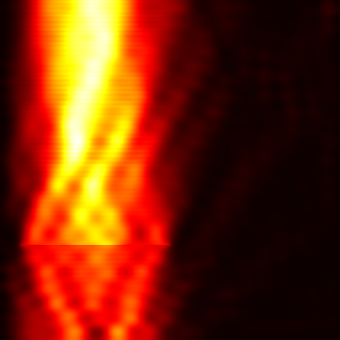
\includegraphics[width=\textwidth]{images/wstep/SUM-nopml-energy.png}
		\caption{}
		\label{fig:wstep-pml-bad}
	\end{subfigure}
	\begin{subfigure}{0.45\textwidth}
		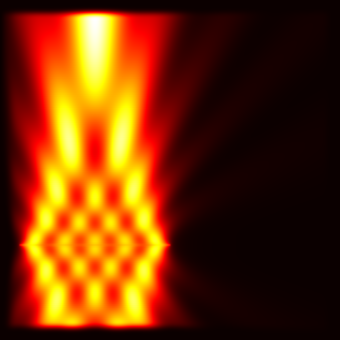
\includegraphics[width=\textwidth]{images/wstep/SUM-pml-energy.png}
		\caption{}
	\end{subfigure}
	\caption{Porównanie wyników symulacji z~propagacją fali E-M w~wolnej przestrzeni dla symulacji w~której brzeg z~warunkiem Dirichleta (a) jest otaczany przez materiał o~$n=1$ , (b) został otoczony obszarem PML}
\end{figure}

Obecnie powszechnie wykorzystywana jest wersja PML nie wymagająca modyfikacji równania falowego, która wyraża PML przez obszar symulacji zajmowany przez jednoosiowy absorbujący materiał anizotropowy. Stąd stosowana nazwa UPML~(ang. uniaxial PML). Pierwotne wyprowadzenie UPML oparte było na analitycznym obliczeniu własności materiału spełniającego warunki absorbcyjności i~zerowego współczynnika odbicia, niezależnie od polaryzacji i~kąta padającego promieniowania E-M  \cite{sacks1995perfectly}. Później przedstawione zostały bardziej elegancie formy wyprowadzenia PML oparte na optyce transformacyjnej~\cite{rappaport1995perfectly}. Podobne wyprowadzenie UPML przytoczone jest w~rozdziale \ref{roz:pml} niniejszej pracy.

Należy również nadmienić, że PML posiada pewne ograniczenia. Jednym z~nich jest zależność współczynnika absorpcji od kąta padania promieniowania E-M. Współczynnik tłumienia jest proporcjonalny do $k_0 \textrm{cos}(\theta)$, gdzie $\theta$ jest kątem padania. Dla kątów bliskich $\frac{\pi}{2}$ tłumienie fali padającej dąży do zera, w~związu z~czym takie fale będą w~znacznym stopniu docierać do brzegu symulacji po odbiciu od którego znów znajdą się w~interesującym nas obszarze. W praktyce, w~symulacjach FDTD można uniknąć tego typu problemów zapewniając odpowiednią odległość symulowanego układu od obszaru PML.


Zasadniczym problemem dotyczącym PML w~symulacjach numerycznych jest odbicie na granicy PML wynikające z~dyskretności siatki obliczeniowej. W celu uniknięcia problemów związanych z~odbiciem numerycznym stosowany w~obliczeniach PML nie jest jednolitym ośrodkiem, ale składa się z~wielu warstw ośrodków o~coraz to większym współczynniku absorpcji.

Niedoskonałością PML, której w~żaden sposób nie można uniknąć jest założenie o~niezmienności ośrodka graniczącego z~PML w~kierunku prostopadłym do PML. Rozwiązaniem pozwalającym uniknąć odbić w~sytuacji, gdy to założenie nie jest spełnione, jest wykorzystanie jedynie absorberów opartych na twierdzeniu adiabateycznym~\cite{oskooi2008failure}.

\subsection{Źródła pola elektromagnetycznego w~symulacjach metodą FDTD}
Ostatnim z~omawianych podstawowych elementów metody FDTD jest wprowadzenie źródeł. Najprostrzym sposobem na realizację tego zadania jest umieszczenie tzw. źródła sztywnego. W takim przypadku w~wybranym punkcie lub punktach symulacji pole elektryczne nie jest obliczane zgodnie z~równaniem \ref{eq:numez-1dfdtd}. Zamiast zależność pola elektrycznego od czasu jest dla niego podana w~sposób analityczny. Tego typu źródło, podobnie jak zadane w~sposób stały warunki brzegowe wprowadza dodatkowe odbicia w~obszarze symulacji.

Innym sposobem wprowadzenia źródła, jest wykorzystanie prawa Ampera z~gęstością prądu
\begin{equation}
\nabla \times \vec{H} = \vec{J} + \varepsilon \frac{\partial \vec{E}}{\partial t},
\label{eq:amper-j}
\end{equation}
gdzie $\vec{J}$ może być rozumiany jako gęstość prądu elektrycznego związana z~przepływem nośników swobodnych w~materiale o~określonej przewodności elektrycznej $\sigma$, ale może też być wykorzystany jako sposób wprowadzenia źródła pola elektrycznego do symulacji. Wprowadzenie źródła addytywnego wymaga wykorzystania innego równania niż prezentowane wcześniej \ref{eq:numez-1dfdtd}. Wyprowadzamy je z~\ref{eq:amper-j} przez zastąpienie pochodnych różnicami skończonymi podobnie jak w~poprzednim wypadku. 



\subsection{Metoda FDTD dla układów o~symetrii walcowej (BOR-FDTD)}
\label{subart:borfdtd}
W przypadku symulacji dotyczącej struktury o~symetrii cylindrycznej możliwe jest zredukowanie problemu trójwymiarowego do problemu dwuwymiarowego. Po zamianie współżędnych na cylindryczne w~równaniach (\ref{eq:fdtd-faraday}) i~(\ref{eq:fdtd-amper}) zależność od kąta $\phi$ separuje się od zmiennych przestrzennych $r$ i~$z$ dając analityczne rozwiązanie w~postaci szeregów zależnych od kąta
\begin{equation}
	\begin{gathered}
	\vec{E}(\vec{r},t)=\sum_{m=0}^{\infty}(\vec{e_u}(r,z,t) \textrm{cos}(m\phi)+\vec{e_v}(r,z,t)\textrm{sin}(m\phi)) \\
	\vec{H}(\vec{r},t)=\sum_{m=0}^{\infty}(\vec{h_u}(r,z,t) \textrm{cos}(m\phi)+\vec{h_v}(r,z,t)\textrm{sin}(m\phi)).
	\end{gathered}
	\label{eq:bor-fields}
\end{equation}

W powyższym wzorze $m$ jest liczbą numerującą azymutalne mody pola E-M, dla określonego modu prowadzenie symulacji wymaga jedynie aktualizowania wartości funkcji $e_u$,$e_v$,$h_u$~i~$h_v$, które to są funkcjami jedynie dwóch zmiennych. Jeżeli rozkład pola na początku symulacji, oraz pól generowanych przez źródła znajdujące się w~obszarze symulacji można rozłożyć na skończoną liczbę elementów sum ze wzorów (\ref{eq:bor-fields}). Wtedy rozwiązując kilka problemów dwu wymiarowych, a następnie stosując zasadę superpozycji pól możemy znaleźć rozwiązanie problemu trójwymiarowego, metodą o~dużo mniejszej złożoności obliczeniowej i~pamięciowej\footnote{Liczba punktów w~symulacji dwuwymiarowej jest kwadratową funkcją rozdzielczości, a w~przypadku obliczeń w~trzech wymiarach sześcienną}.

\begin{figure}
	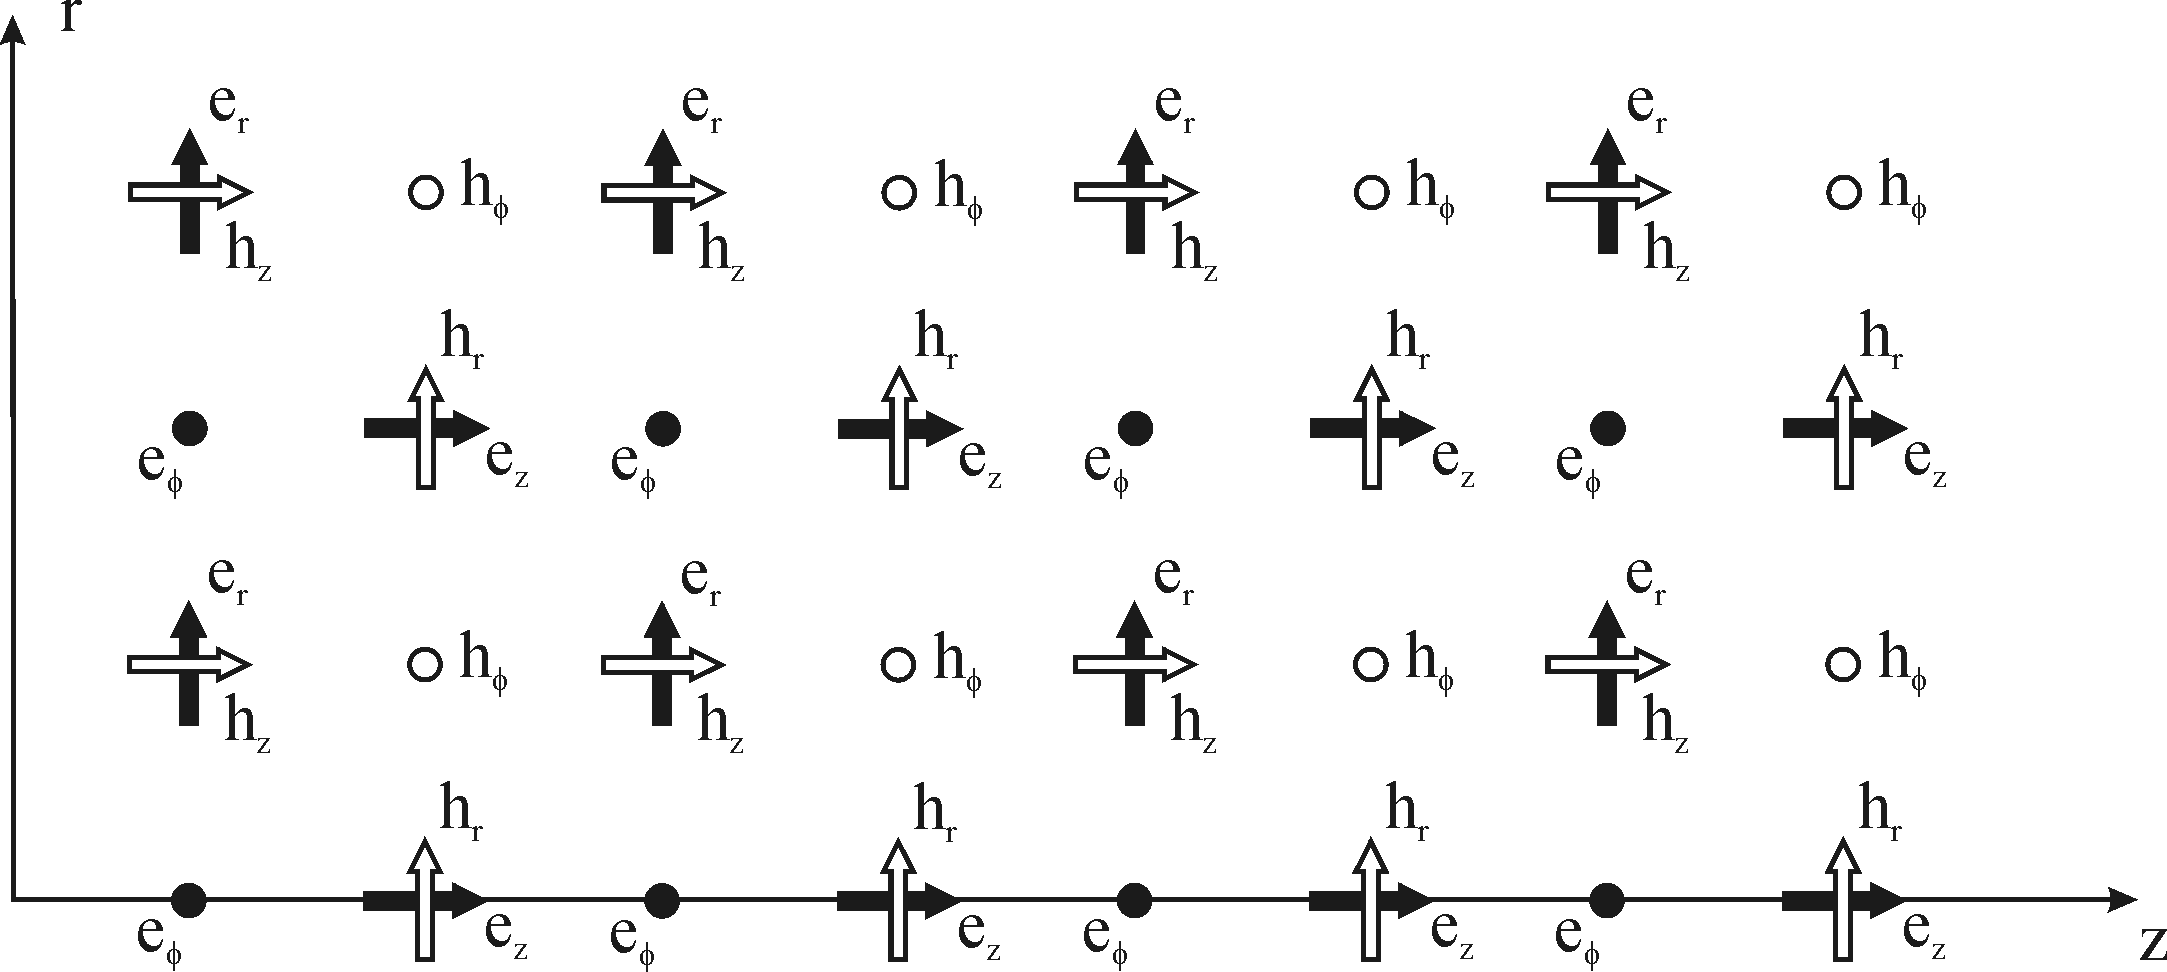
\includegraphics[width=\textwidth]{subart/fdtd/R5_TFSF.png}
	\caption{Przykład dyskretyzacji wykorzystywanej do rozwiązywania równań różniczkowych metodą BOR FDTD \cite{antosiewicz2009wplyw}}
	\label{fig:bor-dysk}
\end{figure}
W przypadku symulacji BOR FDTD stabilność numeryczna wyrażana przez współczynnik Couranta zależy od $m$. Dla $m=0$ największa dopuszczalna wartość współczynnika Couranta $S=\frac{n_min}{\sqrt{2}}$, gdzie $n_min$ oznacza najniższy z~współczynników załamania materiałów w~obszarze symulacji wynosi, dla wyższych modów $S \propto m+1$. 

Ze względu na symetrię układu współrzędnych pola, których punkty dyskretyzacji znajdują się na osi $z$ są tożsamościowo równe zero, poza szczególnymi przypadkami jak $e_z$ dla modu $m=0$, oraz $e_{\phi} i~h_r$ dla m=1 ( dla dyskretyzacji jak na rysunku \ref{fig:bor-dysk}). Ze względu na specjalne traktowanie osi symetrii podczas obliczeń jest to obszar symulacji najbardziej podatny na niestabilności numeryczne. W szczególności, jeśli interesujące nas zjawiska zachodzą zdala od osi optycznej poprawę stabliności uzyskuje się poprzez wymaganie zerowych wartości na kilku rzędach węzłów dyskretyzacji znajdujących się najbliżej osi układu~\cite{OskooiRo10}.

W symulacjach metodą BOR FDTD wynikowe rozkłady pola są dwu wymiarowymi mapami, na których jedna z~osi odpowiada współrzędnej $z$ - konwencjonalnie równoległej do osi symetrii. Druga natomiast współrzędnej $r$ - odległości od osi. 

Przykladowe rozwiązania: fala zanikajaca, plazmon, fala propagujaca?
\section{Systemy liniowe niezmiennicze ze względu na przesunięcia}
Celem ninejszego podrozdziału jest zdefiniowanie pojęcia systemów liniowych, które w~niniejszej pracy znajduje zastosowanie w~analizie zjawisk obrazowania. W ogólności, przez systemem rozumiemy odpowiedniość pomiędzy zestawem funkcji wejściowych, a zestawem funkcji wyjściowych. W przypadku sieci elektrycznych funkcjami wejściowymi jak i~wyjściowymi mogą być zależności napięcia i~natężenia prądu elektrycznego od czasu. Jeżeli ograniczymy opis do systemów deterministycznych, określonemu zestawowi funkcji wejściowych musi odpowiadać dokładnie jeden układ funkcji wyjściowych. Wyjście układu nie musi jednak pozwalać na jednoznaczną identyfikację wejścia, w~szczególności dla wielu stanów wejścia system może nie odpowiadać żadnym wyjściem.

\label{art:lsi}

Matematyczną reprezentacją opisanego systemu, jest operator $S\{\}$, który działając na zbiór funkcji wejściowych $g_i$ tworzy funkcje wyjściowe $f_i$:
\begin{equation}
f_i(\vec{x})=S\{g_i(\vec{x})\}.
\label{eq:system}
\end{equation} 
Warunkiem liniowości systemu opisywanego operatorem $S\{\}$ jest liniowość samego operatora $S\{\}$, która wymaga spełnienia zasady superpozycji matematycznie wyrażonej przez poniższe równanie
\begin{equation}
S\{\alpha p(\vec{x}) + \beta q(\vec{x})\} = \alpha S\{p(\vec{x})\} + \beta S\{q(\vec{x})\},
\label{eq:lin-system}
\end{equation}
spełnione dla dowolnych zespolonych skalarów $\alpha$ i~$\beta$, oraz dowolnych funkcji $p(\vec{x})$ i~$q(\vec{x})$. Zgodnie z~powyższym równaniem, odpowiedź systemu możemy przedstawić jako sumę odpowiedzi na funkcje składowe na które rozłożyliśmy wejście układu. W przypadku zjawisk elektromagnetycznych zasada superpozycji spełniona jest dla amplitud pól elektromagnetycznych w~przypadku promieniowania koherentnego, oraz dla natężeń pól w~przypadku promieniowania nie koherentnego. Do rozkładu funkcji wejściowej na elementarne składowe posłużymy się własnością filtracji delty Diraca
\begin{equation}
g(\vec{x})=\int_{-\infty}^{+\infty} g(\vec{\eta}) \delta(x-\eta) d \vec{\eta}.
\label{eq:dirac-shifting}
\end{equation}
Poszukując funkcji wyjściowej dla układu $S\{\}$ odpowiadającej funkcji wejściowej $g(x)$, wykonujemy podstawienie równania \ref{eq:dirac-shifting} do równania \ref{eq:system} 
\begin{equation}
f(\vec{x})=S \{\int_{-\infty}^{+\infty} g(\vec{\eta}) \delta(\vec{x}-\vec{\eta}) d \vec{\eta} \}.
\label{eq:dirac-shift2}
\end{equation}
Ponieważ funkcja $g(\vec{\eta})$ nie zależy od zmiennych $\vec{x}$, możemy traktować ją jako wagę i~korzystając z~własności superpozycji \ref{eq:lin-system} włączyć operator $S{}$ pod znak całki
\begin{equation}
f(\vec{x})=\int_{-\infty}^{+\infty} g(\vec{\eta})  S\{\delta(\vec{x}-\vec{\eta}) d \vec{\eta} \},
\label{eq:dirac-shift3}
\end{equation}
dla uproszczenia zapisu powyższego równania wprowadzimy funkcję
\begin{equation}
h(\vec{x},\vec{\eta}):=S\{\delta(\vec{x}-\vec{\eta})\}.
\label{eq:imp-resp}
\end{equation}
Powyższa funkcja nazywana jest funkcją odpowiedz impulsowej (ang. impluse response), w~optyce zazwyczaj określa się ją mianem funkcji rozmycia punktu (ang. point-spread function). Korzystając z~wprowadzonego oznaczenia możemy do równania \ref{eq:dirac-shift3}  podstawić definicję \ref{eq:imp-resp}, otrzymując jedną z~podstawowych formuł stosowanych do opisu systemów liniowych, tzw. całkę superpozycji:
\begin{equation}
f(\vec{x})=\int_{-\infty}^{+\infty} g(\vec{\eta})  h(\vec{x},\vec{\eta}) d \vec{\eta} .
\label{eq:sup-int}
\end{equation}
Powyższe równanie wskazuje, że dla opisania odpowiedzi systemu na dowolną funkcję wejściową, niezbędna jest jedynie znajomość funkcji odpowiedzi impulsowej układu. W ogólnym przypadku, funkcja odpowiedzi musi być zdefiniowana dla wszystkich punktowych wzbudzeń w~płaszczyźnie wejściowej. Przykładem analizowanego układu może być np. soczewka oświetlana promieniowaniem niekoherentnym, dla której niezbędnym zestawem informacji potrzebnym do obliczenia natężenia światła w~płaszczyźnie obrazu jest znajomość funkcji odpowiedzi dla wszystkich źródeł punktowych znajdujących się w~płaszczyźnie przedmiotu. 

Szczególne znaczenie dla niniejszej pracy ma kolejna, często spotykana w~zastosowaniach własność układów liniowych określana jako niezmienniczość. W ogólności, może być to np. niezmienniczość systemu elektrycznego w~czasie. 
%Rozumiana jako zależność funkcji odpowiedzi impulsowej $h(t,\tau)$ (gdzie $t$ jest czasem, w~którym poszukiwana jest odpowiedź na impuls elektryczny mający miejsce w~czasie $\tau$) jedynie od różnicy $t-\tau$. Dla układów elektrycznych taka własność jest zazwyczaj spełniona, ponieważ oporniki, kondensatory i~indukcyjności z~których są zbudowane zazwyczaj nie zmieniają swoich własności w~czasie eksperymentów.

Dla układu obrazującego istotną rolę odgrywa izoplanatyczność - niezmienniczość ze względu na przesunięcia, w~wyniku której, funkcja odpowiedzi impulsowej zależy jedynie od odległości pomiędzy położeniem wzbudzenia, a położeniem obrazu
\begin{equation}
h(\vec{x},\vec{\eta})=h(\vec{x}-\vec{\eta}).
\label{eq:shif-inv}
\end{equation}
Powyższa własność zastosowana do układów obrazujących jest więc równoważna stwierdzeniu, że zmiana położenia przedmiotu wpływa jedynie na zmianę położenia jego obrazu. W przypadku niemal wszystkich realnych układów optycznych własność ta nie jest spełniona w~całej przestrzeni położeń, zazwyczaj można jednak obszar podzielić na podobszary, w~których zastosowanie będą miały odpowiednie funkcje $h_i$, natomiast w~ramach pojedynczego podobszaru z~dobrym przybliżeniem stosować można założenie o~izoplanatyczności systemu. Szczególnym przypadkiem obszaru często wykorzystywanego w~analizie obrazowania przez klasyczne elementy optyczne jest otoczenie osi układu, w~stosunku do którego stosuje się omawiane przybliżenie.

Podstawiając równanie (\ref{eq:shif-inv} )do wzoru (\ref{eq:sup-int}) otrzymujemy
\begin{equation}
f(\vec{x})=\int_{-\infty}^{+\infty} g(\vec{\eta})  h(\vec{x}-\vec{\eta}) d \vec{\eta} = g \ast h.
\label{eq:splot}
\end{equation}
W powyższym równaniu $\ast$ oznacza operację splotu. Dzięki sprowadzeniu całki superpozycji dla układów liniowych niezmienniczych ze względu na przesunięcia (ang. LSI - linear shift-invariant) do tej szczególnej postaci, możemy do analizy układów LSI wykorzystać kolejne twierdzenia analizy matematycznej. Ważne znaczenie odgrywa twierdzenie o~splocie, będącego jedną z~podstawowych własności transformaty Fouriera. Zapiszemy powyższe równanie jako
\begin{equation}
F\{f(\vec{\nu})\} = F\{g(\vec{\nu})\} \cdot F\{h(\vec{\nu})\},
\label{eq:transfer-mult}
\end{equation}
gdzie przez $F$ oznaczona została transformata Fouriera, a $\cdot$ oznacza zwykłe mnożenie. W ten sposób znalezienie funkcji wyjściowych układu typu LSI z~obliczania splotu\footnote{Będącego zazwyczaj skomplikowaną operacją analityczną lub wysokiej złożoności operacją numeryczną.} zastąpiliśmy obliczaniem transformaty Fouriera, mnożeniem i~obliczeniem odwrotnej transformaty Fouriera. Transformata Fouriera funkcji odpowiedzi impulsowej ze względu na swoje szczególne znaczenie nazywana jest funkcją przenoszenia $H=F{h}$.

W równaniu (\ref{eq:transfer-mult}) można zauważyć formę zagadnienia własnego opisującego układ typu LSI, w~którym wartości funkcji $H$ dla różnych częstości przestrzennych $\nu$ można interpretować jako wartości własne układu. Funkcjami własnymi są natomiast fale płaskie, ponieważ przeprowadzenie matematycznej operacji transformacji Fouriera jest w~przypadku analizy zjawisk falowych równoważne rozłożeniu funkcji w~bazie fal płaskich.  Kolejnymi wnioskami jakie możemy uzyskać wprost ze wzoru (\ref{eq:transfer-mult}) jest sposób w~jaki układy LSI modyfikują funkcje wejściowe w~postaci fal płaskich. W takim przypadku $G=|A|e^{i \Phi}$ jest po prostu liczbą zespoloną, a układ wprowadza jedynie tłumienie $|A|$ i~stałą modyfikację fazy $\Phi$ padającej nań fali płaskiej~\cite{citeulike:2926459}.

W całej pracy posługując się terminem częstości przestrzennych odnosimy się do podanej powyżej formuły w~której transformacja Fouriera została zastosowana w~stosunku do funkcji położenia, dlatego ze szczególną uwagą należy odróżniać częstości przestrzenne (rozkład w~bazie fal płaskich), od częstotliwości odpowiadającej rozkładowi promieniowania w~bazie fal monochromatycznych.


\section{Modele dyspersji materiałów}
\subsection{Model Lorenza-Drudego}
\label{subart:lorenz-drude}
Powszechnie wykorzystywanym do opisu własności dyspersyjnych materiałów jest model Lorenza-Drudego. \textit{De facto} jest on połączeniem opisu substancji przewodzących (opisywanych modelem Drudego), oraz dielektryków (opisywanych modelem Lorenza). Wyprowadzenie obu modeli opiera się na zastosowaniu zasad mechaniki klasycznej w~stosunku do cząstek naładowanych znajdujących się w~materii. Dla dielektryków przyjmujemy, że są one silnie związane z~węzłami sieci krystalicznej, a ruch każdego ładunku opisuje równanie oscylatora tłumionego, pobudzanego siłą harmoniczną wywoływaną przez zewnętrzne pole elektromagnetyczne~\cite{griffiths1999introduction}:
\begin{equation}
m \frac{d^2 \vec{r}}{dt^2} + m \gamma \frac{d \vec{r}}{dt} + m \omega^2_1 \vec{r} = q \vec{E_0} e^{i \omega t}.
\label{eq:newton-lorenz}
\end{equation}

W powyższym równaniu $m$ nie należy traktować jako masy ładunku, a jako parametr stanowiący tzw. masę efektywną, której wartość można wyznaczyć za pomocą mechaniki kwantowej. Parametry $\omega_1$ i~$\gamma$ możemy zgodnie z~mechaniką klasyczną interpretować odpowiednio jako częstość własną i~współczynnik tłumienia oscylatora. W przypadku substancji o~różnych węzłach sieci krystalicznej, równanie (\ref{eq:newton-lorenz}) należy zapisać osobno dla każdego rodzaju ładunków i~centrów sieci. Rozwiązując powyższe równanie różniczkowe, oraz korzystając z~definicji polaryzacji możemy wyznaczyć przenikalność elektryczną ośrodka nieprzewodzącego jako:

\begin{equation}
\varepsilon = 1 + \frac{N_o q^2}{\varepsilon_0 m} \sum_j \frac{f_j}{\omega_j^2 - \omega - i~\gamma_j}.
\label{eq:lorenz}
\end{equation}

Wprowadzone w~powyższym równaniu współczynniki $f_j$ opisują tzw. siłę oscylatora, związaną z~prawdopodobieństwem przejść między stanami cząstek opisywanego materiału. Wprowadzony parametr $N_o$ opisuje koncentrację oscylatorów.  W przeciwieństwie do izolatorów elektrycznych opis metali musi przede wszystkim uwzględnić istnienie nośników swobodnych. Zaniedbując oddziaływanie ładunków swobodnych ze sobą i~zakładając, że ich zderzenia z~wierzchołkami sieci krystalicznej mają charakter w~pełni przypadkowy możemy ich klasyczne równanie ruchu zapisać jako:

\begin{equation}
m \frac{d^2\vec{r}}{dt} + m \gamma \frac{d\vec{r}}{dt} = q \vec{E_0}e^{i\omega t}.
\label{eq:newton-drude}
\end{equation}

W powyższym równaniu wprowadzona siła oporu $m \gamma \vec{v}$ wynika ze zderzeń z~węzłami sieci krystalicznej. Rozwiązanie powyższego równanie prowadzi do następującego wyrażenia na przenikalność dielektryczną

\begin{equation}
\varepsilon= 1 - \frac{\omega_p^2}{\omega^2+i\omega \gamma},
\label{eq:drude}
\end{equation}

w którym wprowadzona wartość $\omega_p$ to częstość plazmowa, opisywana wzorem:

\begin{equation}
\omega_p = \sqrt{\frac{N q^2}{\epsilon_0 m}},
\label{eq:omega-plazmowa}
\end{equation}
gdzie $N$ jest koncentracją swobodnych nośników o~ładunku $q$. Im większa koncentracja nośników swobodnych, tym większa jest częstość plazmowa opisywanego metalu.  Dla częstotliwości z~zakresu optycznego $\gamma<<\omega$ co jest odzwierciedleniem faktu, że droga swobodna elektronów w~paśmie przewodnictwa jest znacznie większa od rozważanych długości fali. Zgodnie z~równaniem  (\ref{eq:drude}) oznacza to, że dla światła widzialnego decydującą rolę dla własności metali ma część rzeczywista $\varepsilon$, która jest dodatnia tylko dla $\omega>\omega_p$. Dla takich częstotliwości równanie falowe w~metalach będzie mieć rozwiązanie w~postaci fal poprzecznych. Fizyczną interpretację $\omega_p$ znaleźć można w~rozwiązaniu równania (\ref{eq:newton-drude}). Jest to częstość własna drgań podłużnych elektronów swobodnych. Częstość plazmowa jest natomiast podstawą dla wprowadzenia pojęcia plazmonu objętościowego, stanowiącego kwant omawianych drgań.

Ponieważ polaryzacja jest sumą efektywnych momentów dipolowych przypadających na jednostkę objętości, to wkłady do polaryzacji pochodzące od oddziaływań z~elektronami w~paśmie przewodnictwa i~jonami sieci krystalicznej podlegają dodawaniu. Dlatego model przenikalności elektrycznej materiałów uwzględniający oba te zjawiska, jest sumą wkładów pochodzących z~równań (\ref{eq:lorenz}) i~(\ref{eq:drude}). Zazwyczaj model materiałowy dopasowywany jest do danych eksperymentalnych jedynie w~ograniczonym zakresie. Ze względu na to większość rezonansów ze wzoru (\ref{eq:lorenz}) może zostać zastąpionych stałą wartością zwyczajowo określaną jako $\varepsilon_\infty$, a ostateczny wzór przyjmuje postać
\begin{equation}
\varepsilon(\omega)=\varepsilon_\infty- \frac{\omega_p^2}{\omega^2+i\omega\gamma} +\frac{Nq^2}{\varepsilon_0 m} \Sigma_j \frac{f_j}{\omega_j^2-\omega^2-i\gamma_j\omega}
\label{eq:lorenz-drude}
\end{equation}

\section{Przybliżenie ośrodka efektywnego}
\label{subart:effmedium}

\begin{equation}
	\label{eq:effmedium}
\end{equation}


